% Adjust these for the path of the theme and its graphics, relative to this file
%\usepackage{beamerthemeFalmouthGamesAcademy}
\usepackage{../../beamerthemeFalmouthGamesAcademy}
\usepackage{multimedia}
\usepackage{soul}
\usepackage{tikz}
\usepackage{verbatim}
\graphicspath{ {../../} }

% Default language for code listings
\lstset{language=C++,
        morekeywords={each,in,nullptr}
}

% For strikethrough effect
\usepackage[normalem]{ulem}
\usepackage{wasysym}

\usepackage{pdfpages}

% http://www.texample.net/tikz/examples/state-machine/
\usetikzlibrary{arrows,automata}

\newcommand{\modulecode}{COMP260}\newcommand{\moduletitle}{Distributed Systems}\newcommand{\sessionnumber}{5}

\begin{document}
\title{\sessionnumber: \normalsize{Human-Centred Design for AR/VR}}
\subtitle{\modulecode: \moduletitle}

\frame{\titlepage} 

% ASSIGNMENT BRIEFS
\begin{frame}
	\frametitle{Assignment Briefs}
	\begin{itemize}
		\item \textbf{Evaluate} an existing screen-based game interface
		\item \textbf{Design} and \textbf{develop} an interface that incorporates either AR or VR
		\item \textbf{Produce} a journal detailing your research into virtual and augmented reality
	\end{itemize}
\end{frame}

% LEARNING OUTCOMES
\begin{frame}
	\frametitle{Virtual and Augmented Reality Overview:}
	
	\textbf{Learning Outcomes:}
	
	\begin{itemize}
		\item \textbf{Explain} the difference between augmented \& virtual reality. 
		\item \textbf{Discuss} the various forms of haptic feedback.
		\item \textbf{List} and \textbf{describe} the key components that make up the hardware side of reality systems.	
	\end{itemize}
\end{frame}

\begin{frame}
	\frametitle{A Word of Warning}
	AR/VR are both emerging technologies and thus, they borrow language from other similar disciplines such as game development, film studies and 3D design. This appropriation of lexicons can be confusing and there will be some overlap in relation to key terms and definitions.
\end{frame}

\begin{frame}
	\begin{figure}
		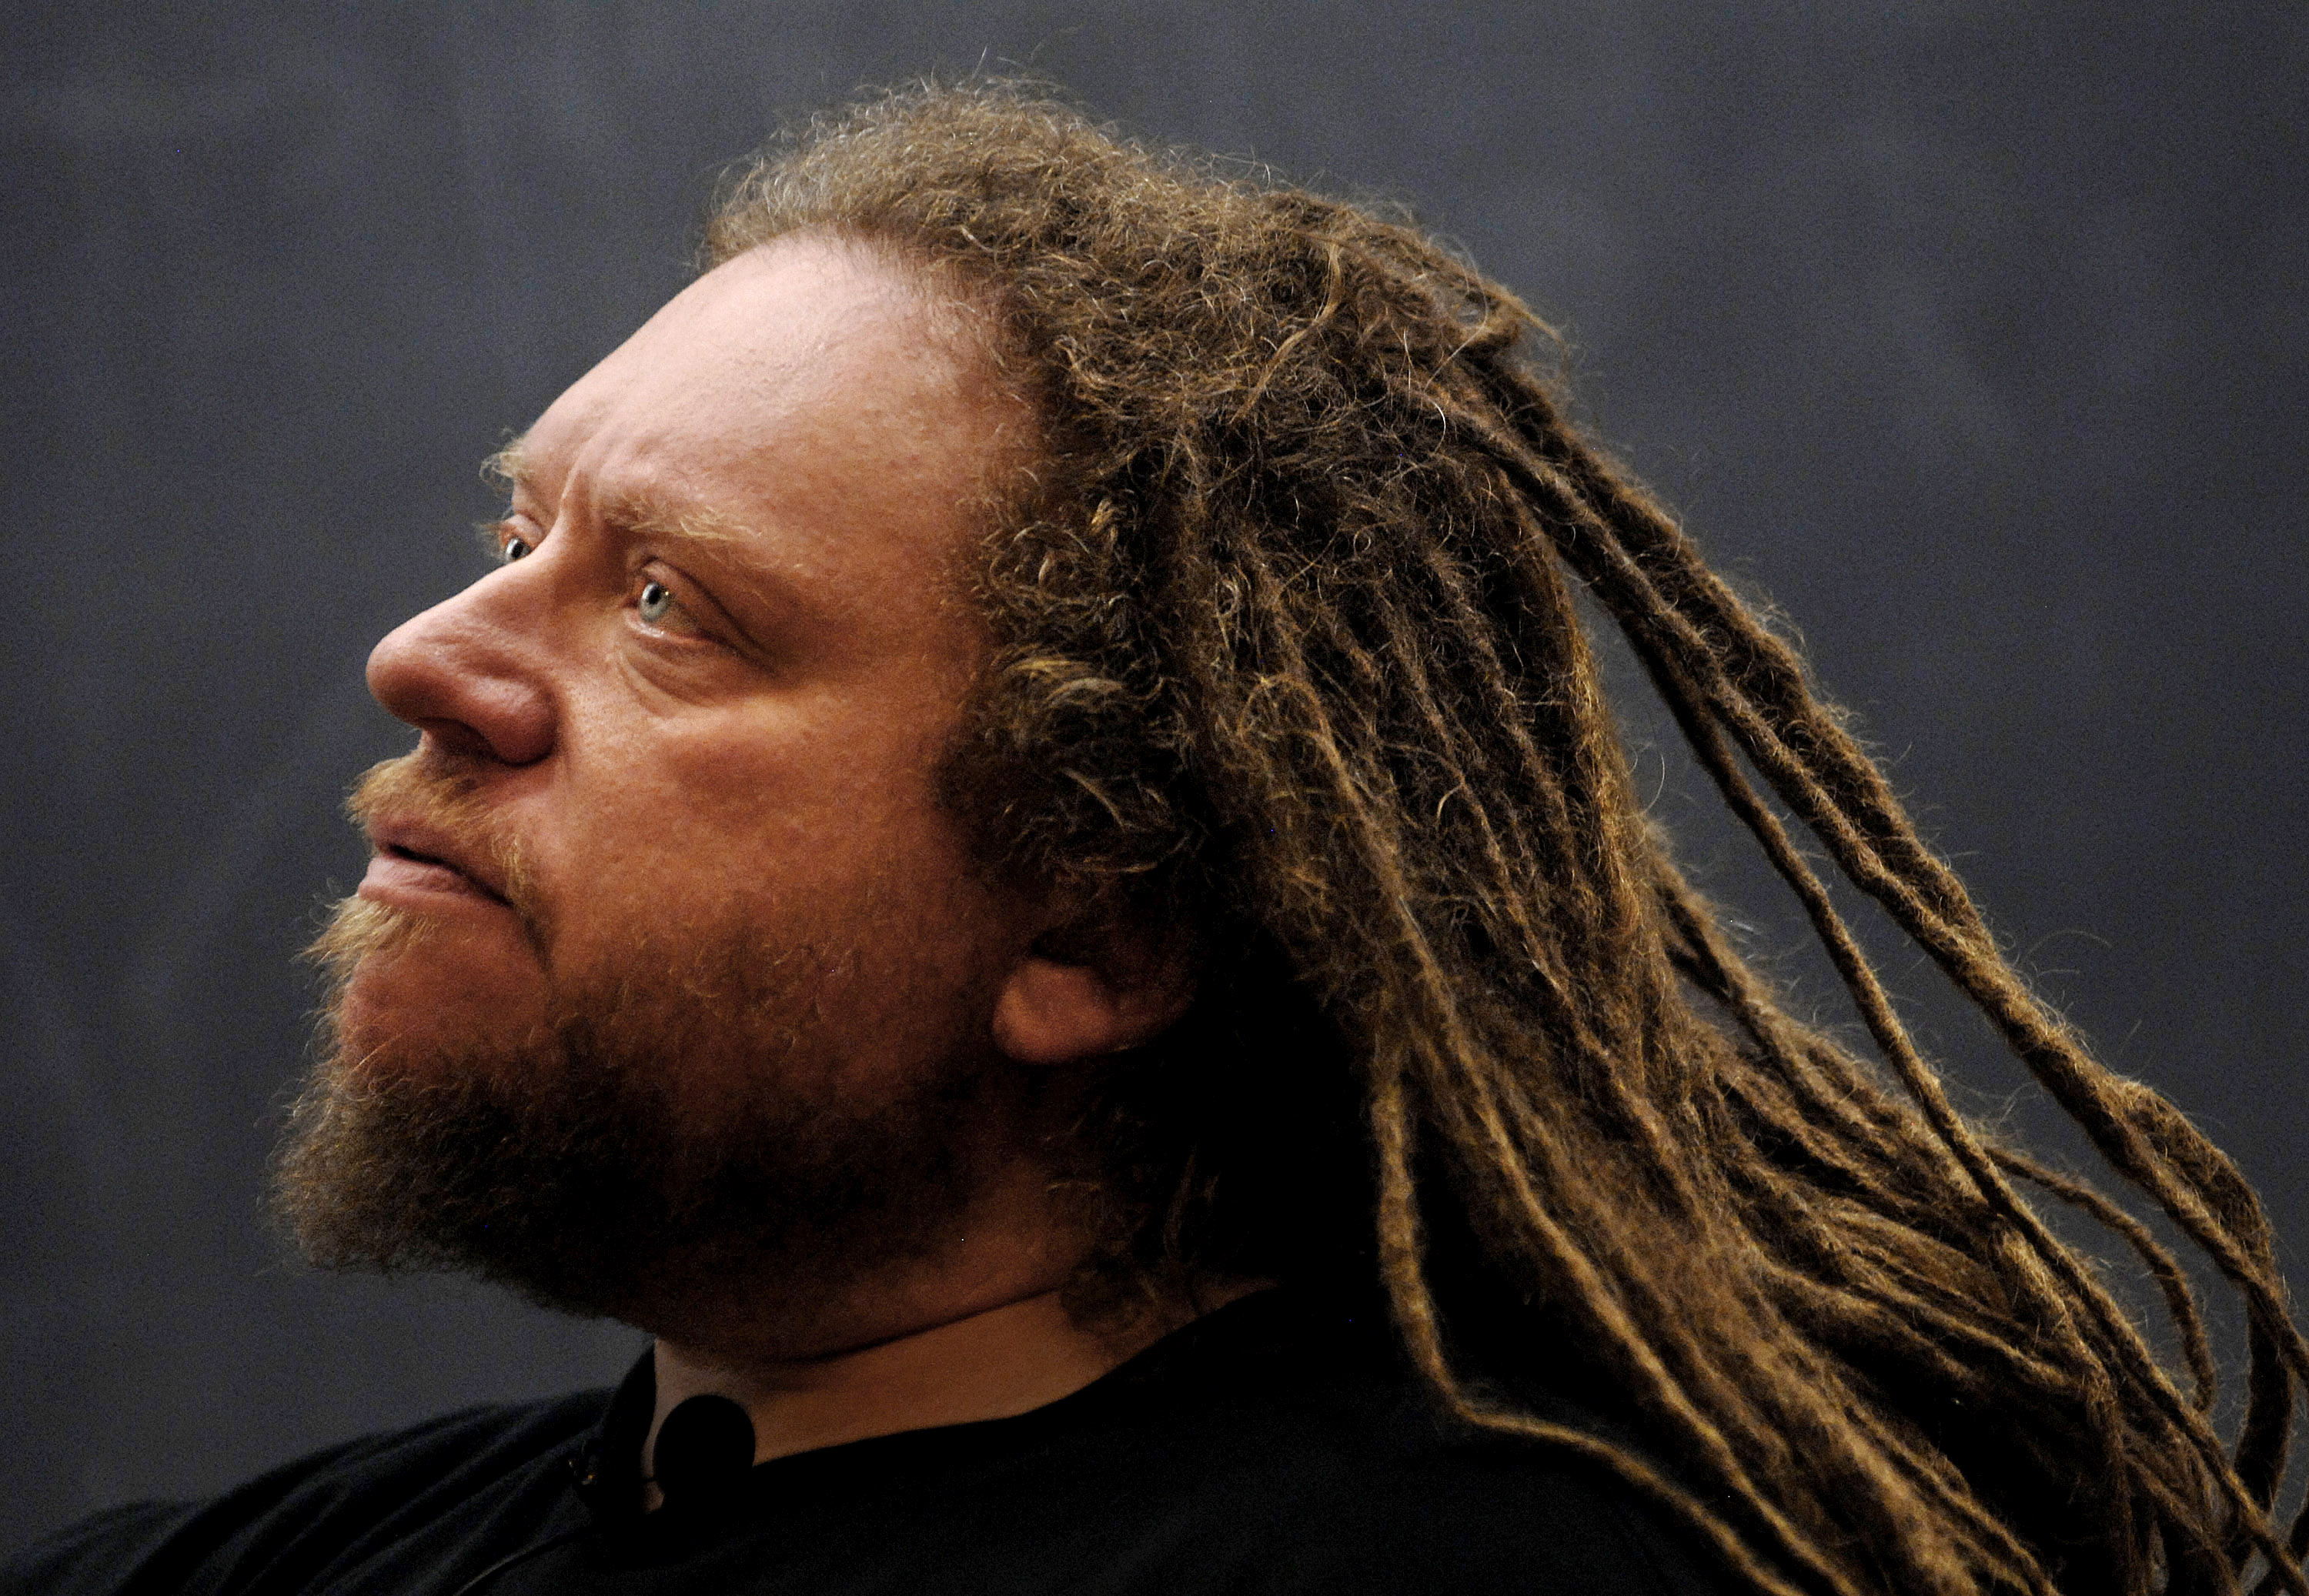
\includegraphics[scale=0.3]{assets/lanier.jpg}
	\end{figure}
	The term `virtual reality' was coined by Jaron Lanier in 1987 during a period of intense research activity into this form of technology.
	
\end{frame}

\begin{frame}
	\begin{figure}
		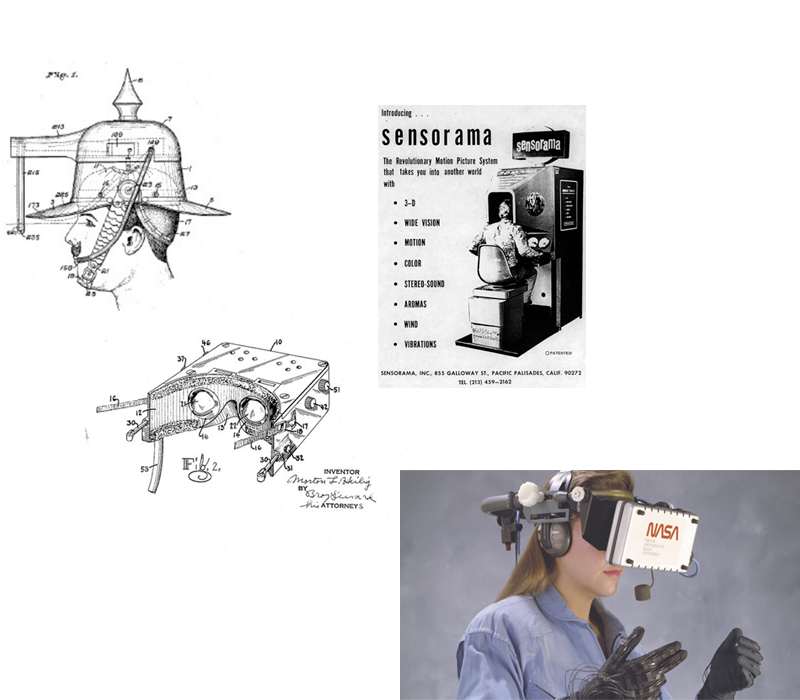
\includegraphics[scale=.6]{assets/history.png}
		\caption{\tiny{Left to Right - Pratt's head-mounted targeting interface, Heilig's Stereoscope TV Apparatus \& Sensorama, NASA's VIEW System} }
	\end{figure}
\end{frame}

\begin{frame}
	\frametitle{Forms of Reality}
	\begin{figure}
		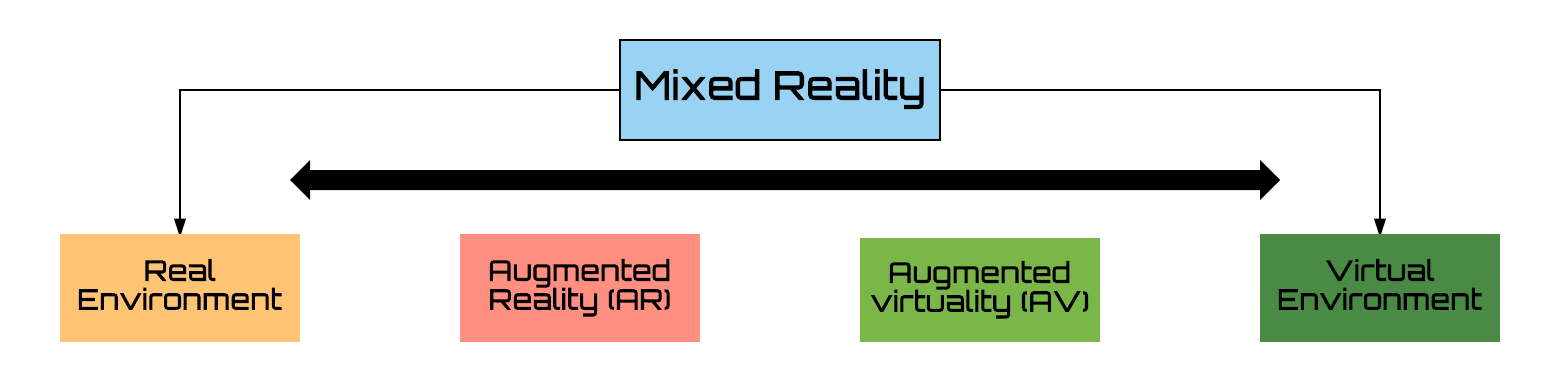
\includegraphics[scale=.2]{assets/continuum.png}
		\caption{The Virtuality Continuum - Milgram \& Kishino}
	\end{figure}
\end{frame}

% Hands up who has had a go with....
% run through some of the introduction from book.

%REALITY SYSTEMS
\begin{frame}
	\frametitle{Reality Systems - Hardware}
	
	\begin{columns}
		
		\begin{column}{0.5\textwidth}
			\textbf{Display Types:}
			\begin{itemize}
				\item Head-Mounted Displays
				\item World-Fixed Displays
				\item Hand-held Displays
			\end{itemize}
		\end{column}
		
		\begin{column}{0.5\textwidth}

			\textbf{Audio:}
			Spatialised Audio is preferred
			\begin{itemize}
				\item Headphones - more immersive.
				\item surround sound speakers.
			\end{itemize}
			
		\end{column}
		
	\end{columns}
\end{frame}

\begin{frame}
	\frametitle{Head-Mounted Displays (HMD)}
	\begin{figure}
		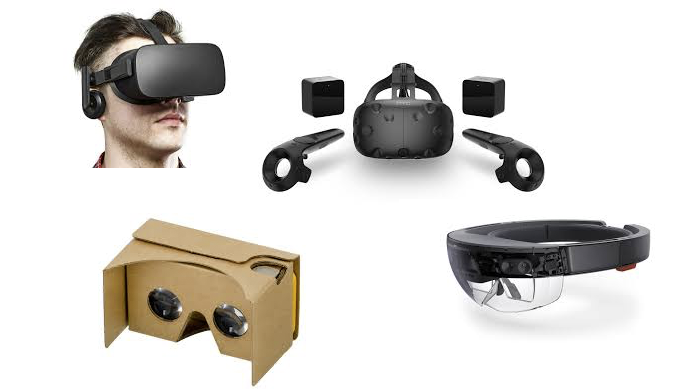
\includegraphics[scale=0.4]{assets/hmd.png}
	\end{figure}
\end{frame}

\begin{frame}
	\frametitle{World-Fixed Display}
	\begin{figure}
		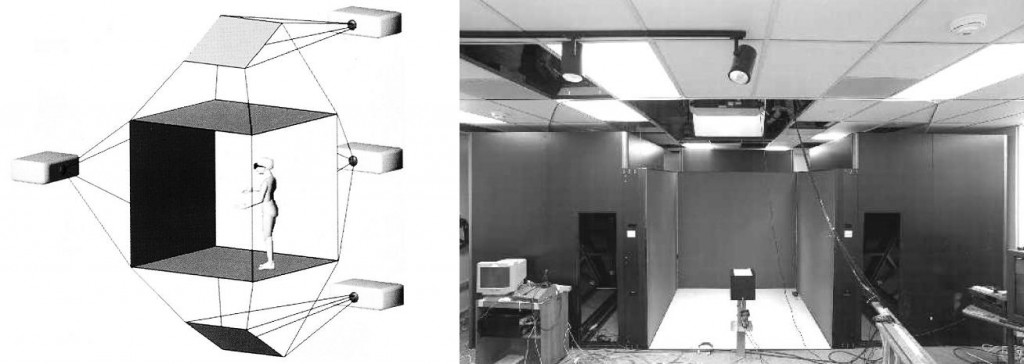
\includegraphics[scale=0.3]{assets/cave.jpg}
		\caption{Cave VR environment: A lifelike visual display is created by projectors positioned outside the CAVE and controlled by physical movements from a user inside the CAVE.}
	\end{figure}
\end{frame}

\begin{frame}
	\frametitle{Hand-held displays}
	Have a guess at the example I chosen?
	\pause
	\begin{figure}
		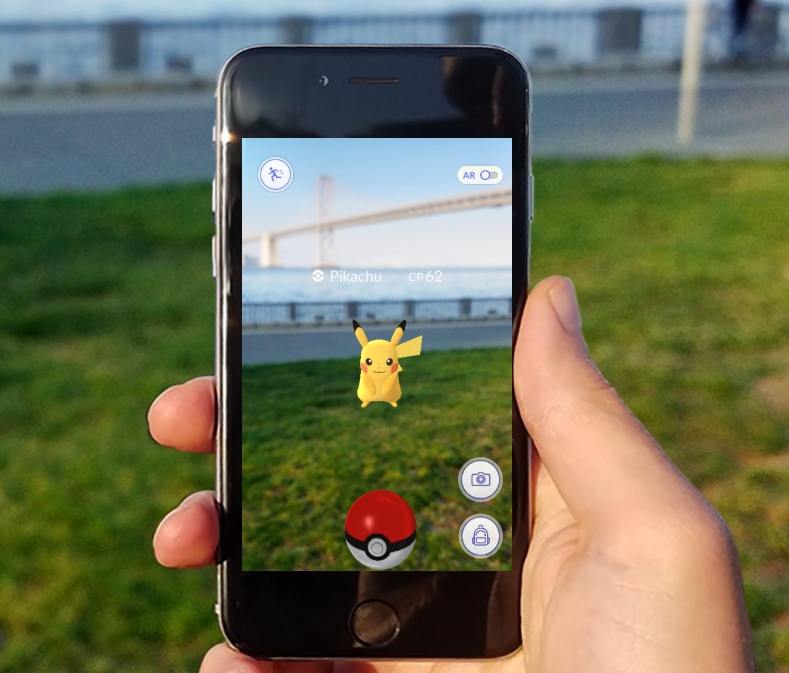
\includegraphics[scale=0.25]{assets/pgo.png}
		\caption{Pokemon Go}
	\end{figure}
	
\end{frame}

%TRACKING
\begin{frame}
	\frametitle{Tracking}
	\begin{itemize}
		\item Accelerator \& Gyro embedded in HMD
		\item Leap motion - Hand Tracking
		\item Eye Tribe (Foveated rendering)
		\item Fiducials Markers
		\item Kinect2 - Skeleton Tracking
		\item Valve?s Lighthouse Tracking Sensors
	\end{itemize}
\end{frame}

\begin{frame}
	\frametitle{Haptics}
	Haptics are the artificial forces between virtual objects and the user.
	\vspace{.2in}
	
	\textbf{Passive -}
	real-world physical objects that match the shapes of a virtual objects. (Doors, ledges, pillars... )
	\vspace{.2in}
	
	\textbf{Active -} Haptics can be dynamically controlled by the computer to provide a feeling of a wide range of simulated virtual objects.
	
\end{frame}

\begin{frame}
	\begin{figure}
		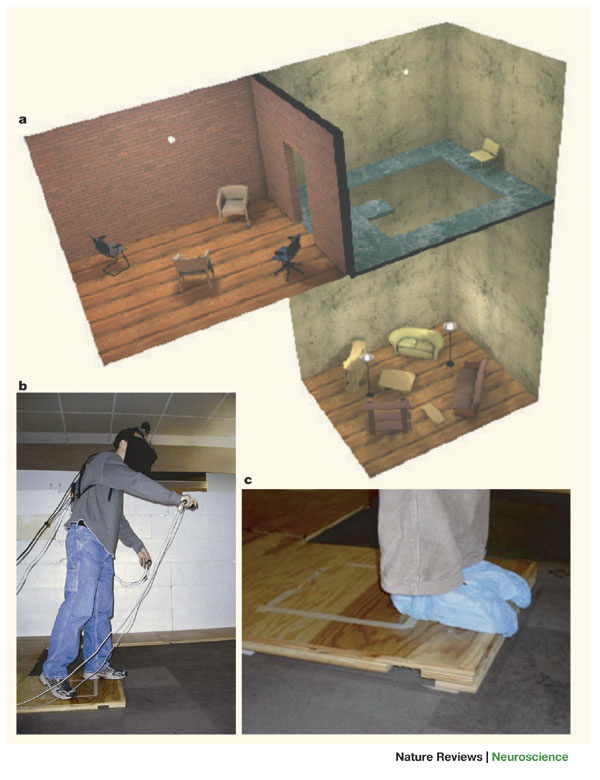
\includegraphics[scale=0.25]{assets/thepit.png}
		\caption{University of North Carolina - Pit Experiment}
	\end{figure}
\end{frame}

\begin{frame}
	
	\frametitle{Tactile Haptics}
	
	\begin{itemize}
		\item Vibrotactile - vibration passed directly or indirectly to the skin
		\item Electrotactile - electrodes passing current through the skin
		\item Proprioceptive force - provides a sense of limb movement and muscular resistance
	\end{itemize}	
	
\end{frame}

\begin{frame}
	\frametitle{Self-Grounded vs. World-Grounded Haptics}
	\begin{figure}
		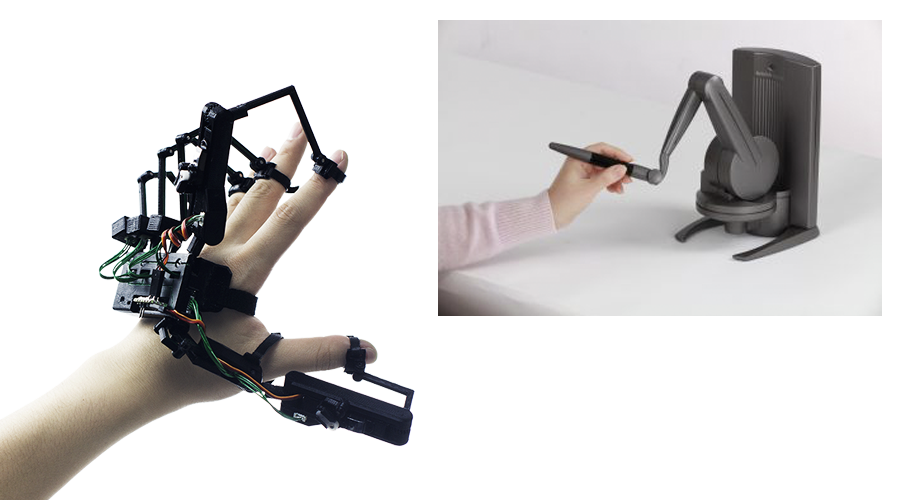
\includegraphics[scale=0.3]{assets/self-world.png}
		\caption{DexmoF2 \& Sensable's Phantom Haptic System}
	\end{figure}
	
\end{frame}

\begin{frame}
	\frametitle{Motion Platforms}
	A motion platform is a hardware device that moves the entire body resulting in a sense of physical motion and gravity. 
	\vspace{.2in}
	
	
	These systems can convey a sense of orientation, vibration, acceleration and jerking.	
	\vspace{.2in}
	
	
	[Examples]
	
\end{frame}

{
      \begin{frame}[plain]
        \begin{tikzpicture}[remember picture,overlay]
            \node[at=(current page.center)] {
                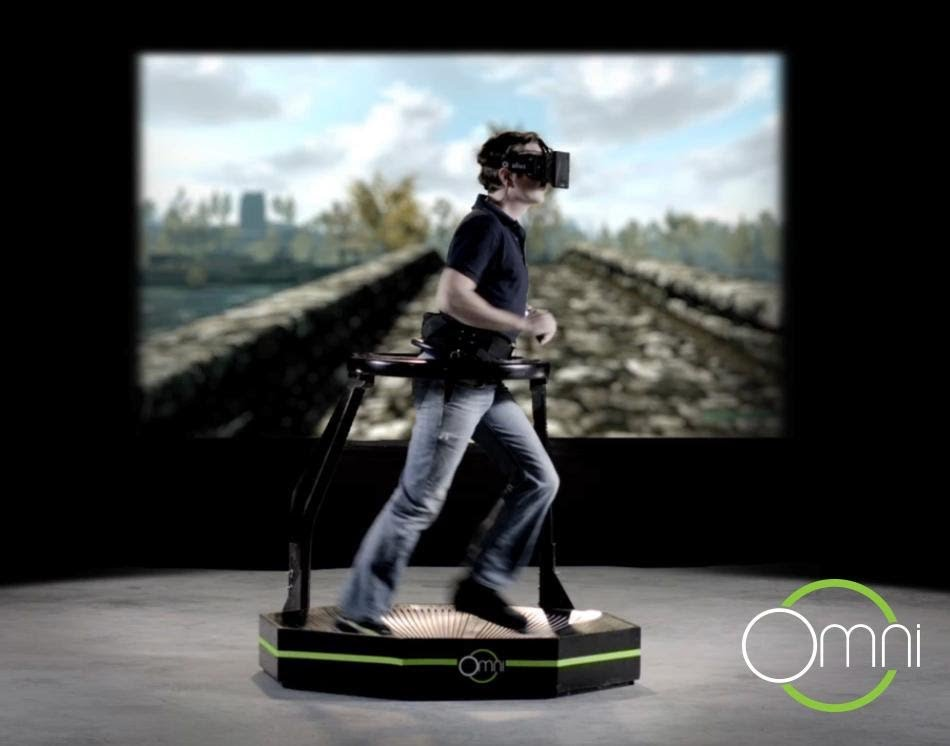
\includegraphics[width=\paperwidth]{assets/virtuix}
            };
        \end{tikzpicture}
     \end{frame}
}

{
      \begin{frame}[plain]
        \begin{tikzpicture}[remember picture,overlay]
            \node[at=(current page.center)] {
                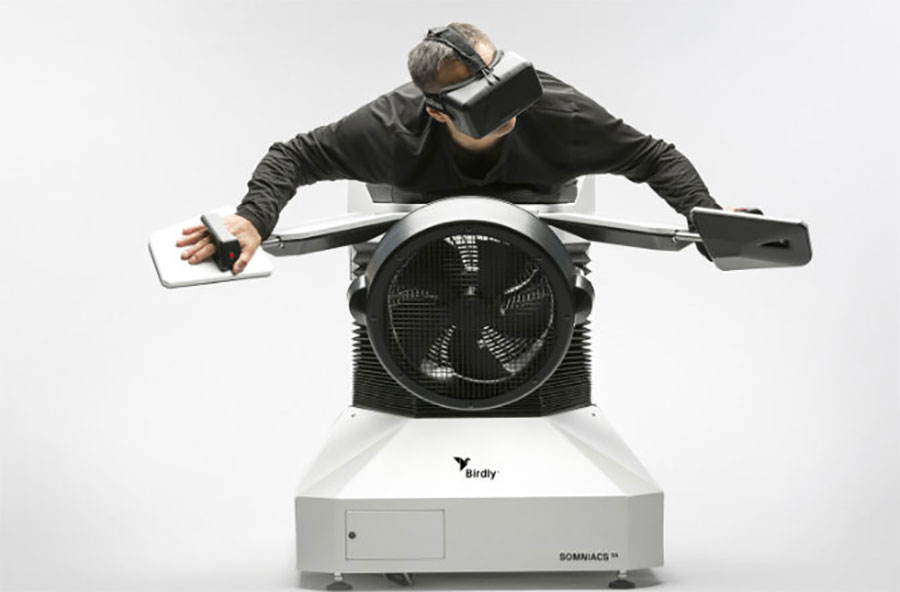
\includegraphics[width=\paperwidth]{assets/birdy}
            };
        \end{tikzpicture}
     \end{frame}
}


\begin{frame}
	\frametitle{Human-Centred Design:}
	
	\textbf{Learning Outcomes:}
	
	\begin{itemize}
		\item \textbf{explain} the importance of placing the user at the centre of the design process
		\item \textbf{briefly} describe and compare different user-centred design techniques
		\item \textbf{demonstrate} a knowledge of the principles of user-centred design.	
		\item \textbf{acknowledge} that sophisticated/eloquent solutions are less important than great user experiences. 
	\end{itemize}
\end{frame}



% CONTINUOUS DISCOVERY 
\begin{frame}
	\frametitle{Continuous Discovery}
	Continuous discovery is the on-going process of engaging users during the design and development process. 
	\begin{itemize}
		\item \pause You can never know everything in advance of a project.
		\item \pause Waiting until the end of a build to find out that something doesn't work is unsustainable. 
		\item \pause Change is inevitable.
		\item \pause Failures are an inevitable outcome of creativity and innovation. 
	\end{itemize}
\end{frame}	

% ITERATION CYCLE
\begin{frame}
	\frametitle{Iteration}
	\begin{figure}
		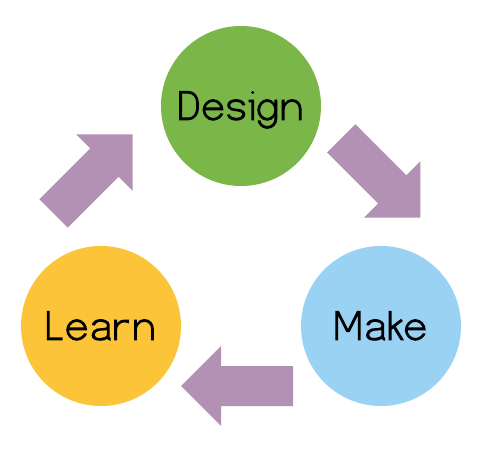
\includegraphics[scale=0.4]{assets/iteration.png}
		\caption{The Iteration Cycle}
	\end{figure}
\end{frame}



% DEFINE STAGE
\begin{frame}
	\frametitle{ Design/Define Stage}
	This stage attempts to answer the question, `what do we want to make?' and includes everything from the high-level vision to listing requirements. All parts of the define stage should be described from the users point of view and easily understood by all. 
	\pause
	\begin{columns}
		\begin{column}{0.5\textwidth}
			\begin{itemize}
				\item Vision
				\item Objectives 
				\item Key Players				
				\item Time \& Costs
				\item Risks
			\end{itemize}
   		\end{column}
		
		\begin{column}{0.5\textwidth}  
			\begin{itemize}
				\item Assumptions
				\item Constraints
				\item Personas		
				\item User Stories
				\item Story Boards
			\end{itemize}
		\end{column}
	\end{columns}
\end{frame}

\begin{frame}
	\frametitle{\textbf{ASK QUESTIONS}}
	\begin{itemize}
		\item Feedback is crucial at the define stage. 
		\item Ask lots of questions.
		\item Do not trust assumptions. 
		\item Common misconception.
	\end{itemize}
\end{frame}

\begin{frame}
	\begin{center}
		\Huge{Analysis Paralysis }
	\end{center}
\end{frame}


% MAKE STAGE
\begin{frame}
	\frametitle{Make Stage}
	This stage answers the question, `how do we make it?' and then proceeds to make it. Each iteration of the make stage should take the project from basic sketches and minimal prototypes, closer and closer to the final product. 
	
\pause
	\begin{itemize}
		\item Use Cases
		\item Block Diagrams 
		\item Sketches				
		\item Prototypes
		\item Class Definitions
		\item Hardware and Software implementation   		
	\end{itemize}
\end{frame}

\begin{frame}
	\frametitle{Prototypes}
	A prototype is a simplistic implementation of what is trying to be accomplished without being overly concerned with aesthetics or perfection. Design prototypes are defined by their level of fidelity, or resolved finish. 
	\begin{figure}
		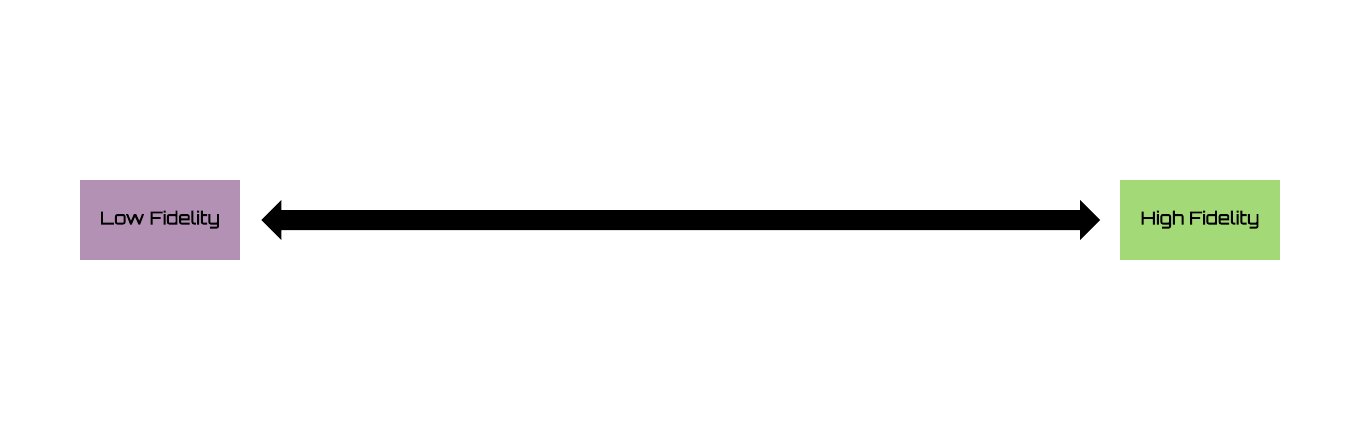
\includegraphics[scale=0.23]{assets/prototype.png}
		\caption{The Prototype Continuum}
	\end{figure}
\end{frame}


\begin{frame}
	\frametitle{Learn Stage}
	Utilises VR experts, subject matter experts, experiment design experts, statisticians and the end-user to ensure that you are doing the right things to maximise learning. 
	
	\vspace{.2in}
	This is the stage that we are mostly concerned with when approaching assignment COMP210 1.
\end{frame}

\begin{frame}
	\frametitle{Research Factors}
	\begin{itemize}
		\item Lab vs. field
		\item Granularity
		\item Summative or formative
		\item Objective vs. subjective
	\end{itemize}
\end{frame}

\begin{frame}
	\frametitle{Research / Evaluation Methods}
	
	\huge Qualitative vs. Quantitative 
\end{frame}

\begin{frame}
	\frametitle{Qualitative}
	Research that aims to gain a deeper understanding of underlying reasons, opinions, and motivations and provide insights into a particular scenario or problem.  Qualitative Research is primarily exploratory research and usually leads into quantitative research 
	\end{frame}

\begin{frame}
	\frametitle{Quantitative}
	Research that aims to quantify the problem or scenario through collecting numerical data that can be analysed and interrogated using statistics. Quantitative research is great for quantifying opinions, behaviour, attitudes and other defined variables.
	\end{frame}	

\begin{frame}
	\frametitle{Methods}
	\begin{itemize}
		\item Usability Testing
		\item Eye Tracking
		\item Cognitive Walkthrough
		\item Heuristic Evaluation
		\item Focus Groups
		\item User-Experience Questionnaire
		\item Task and reaction measurement Galvanic Skin Response
		\item Observation Studies
		\item Think-aloud protocols
	\end{itemize}
\end{frame}

\begin{frame}
	\frametitle{Socrative}
	Room: WN2DMYEVN
\end{frame}

\begin{comment}
\begin{frame}
	\frametitle{Communication and Attitude}
	\begin{itemize}
		\item	\pause Never blame or belittle users or their opinions/interactions with your product. Doing so will shut them down emotionally where they will not effectively provide feedback.
		\item	\pause  Actively investigate difficulties to determine how the project can improve. 
		\item	\pause  Do not assume what works for you will work for everyone else. 
		\item	\pause  When someone points out a problem that you are already aware of, thank them for noticing and then encourage them to continue looking for problems. 
		\item	\pause  Instead of using words like failure, talk about learning. 
	\end{itemize}
\end{frame}
\end{comment}

\end{document}
